
%(BEGIN_QUESTION)
% Copyright 2012, Tony R. Kuphaldt, released under the Creative Commons Attribution License (v 1.0)
% This means you may do almost anything with this work of mine, so long as you give me proper credit

This Ethernet network has a problem in it somewhere:

$$\includegraphics[width=15.5cm]{i02123x01.eps}$$

\begin{itemize}
\item{} 1 can ``ping'' 3
\item{} 4 can ``ping'' {\tt www.google.com}
\item{} 4 can ``ping'' 5 
\item{} 2 cannot ``ping'' {\tt www.google.com}
\end{itemize}

\vskip 10pt

An excellent diagnostic strategy is to trace paths of data flow in a complex system, looking for places of intersection.  Successful paths prove all points along the pathway are functioning.  Places of overlap between unsuccessful paths prove that section is suspect.

Apply this strategy to the problem at hand, and use the results to narrow the field of possible faults.

\vskip 10pt

Also, identify a good ``next ping'' test to do.


\underbar{file i02123}
%(END_QUESTION)





%(BEGIN_ANSWER)

``Good'' paths shown in bright green, ``bad'' paths shown in bright red:

$$\includegraphics[width=15.5cm]{i02123x02.eps}$$

Suspect components include 2, cable between 2 and hub A, cable between hub A and router.

\vskip 10pt

A good ``next ping'' test to do is to try pinging 1 or 3 from 2: that would test 2 as well as the cable between 2 and hub A.  An alternative test would be to ping 4 or 5 from 1 or 3: that would test the cable between hub A and the router.

%(END_ANSWER)





%(BEGIN_NOTES)


%INDEX% Networking, Ethernet: troubleshooting using "ping"

%(END_NOTES)


